\documentclass[twoside]{book}

% Packages required by doxygen
\usepackage{fixltx2e}
\usepackage{calc}
\usepackage{doxygen}
\usepackage[export]{adjustbox} % also loads graphicx
\usepackage{graphicx}
\usepackage[utf8]{inputenc}
\usepackage{makeidx}
\usepackage{multicol}
\usepackage{multirow}
\PassOptionsToPackage{warn}{textcomp}
\usepackage{textcomp}
\usepackage[nointegrals]{wasysym}
\usepackage[table]{xcolor}

% NLS support packages
\usepackage[ngerman]{babel}

% Font selection
\usepackage[T1]{fontenc}
\usepackage[scaled=.90]{helvet}
\usepackage{courier}
\usepackage{amssymb}
\usepackage{sectsty}
\renewcommand{\familydefault}{\sfdefault}
\allsectionsfont{%
  \fontseries{bc}\selectfont%
  \color{darkgray}%
}
\renewcommand{\DoxyLabelFont}{%
  \fontseries{bc}\selectfont%
  \color{darkgray}%
}
\newcommand{\+}{\discretionary{\mbox{\scriptsize$\hookleftarrow$}}{}{}}

% Page & text layout
\usepackage{geometry}
\geometry{%
  a4paper,%
  top=2.5cm,%
  bottom=2.5cm,%
  left=2.5cm,%
  right=2.5cm%
}
\tolerance=750
\hfuzz=15pt
\hbadness=750
\setlength{\emergencystretch}{15pt}
\setlength{\parindent}{0cm}
\setlength{\parskip}{3ex plus 2ex minus 2ex}
\makeatletter
\renewcommand{\paragraph}{%
  \@startsection{paragraph}{4}{0ex}{-1.0ex}{1.0ex}{%
    \normalfont\normalsize\bfseries\SS@parafont%
  }%
}
\renewcommand{\subparagraph}{%
  \@startsection{subparagraph}{5}{0ex}{-1.0ex}{1.0ex}{%
    \normalfont\normalsize\bfseries\SS@subparafont%
  }%
}
\makeatother

% Headers & footers
\usepackage{fancyhdr}
\pagestyle{fancyplain}
\fancyhead[LE]{\fancyplain{}{\bfseries\thepage}}
\fancyhead[CE]{\fancyplain{}{}}
\fancyhead[RE]{\fancyplain{}{\bfseries\leftmark}}
\fancyhead[LO]{\fancyplain{}{\bfseries\rightmark}}
\fancyhead[CO]{\fancyplain{}{}}
\fancyhead[RO]{\fancyplain{}{\bfseries\thepage}}
\fancyfoot[LE]{\fancyplain{}{}}
\fancyfoot[CE]{\fancyplain{}{}}
\fancyfoot[RE]{\fancyplain{}{\bfseries\scriptsize Erzeugt von Doxygen }}
\fancyfoot[LO]{\fancyplain{}{\bfseries\scriptsize Erzeugt von Doxygen }}
\fancyfoot[CO]{\fancyplain{}{}}
\fancyfoot[RO]{\fancyplain{}{}}
\renewcommand{\footrulewidth}{0.4pt}
\renewcommand{\chaptermark}[1]{%
  \markboth{#1}{}%
}
\renewcommand{\sectionmark}[1]{%
  \markright{\thesection\ #1}%
}

% Indices & bibliography
\usepackage{natbib}
\usepackage[titles]{tocloft}
\setcounter{tocdepth}{3}
\setcounter{secnumdepth}{5}
\makeindex

% Hyperlinks (required, but should be loaded last)
\usepackage{ifpdf}
\ifpdf
  \usepackage[pdftex,pagebackref=true]{hyperref}
\else
  \usepackage[ps2pdf,pagebackref=true]{hyperref}
\fi
\hypersetup{%
  colorlinks=true,%
  linkcolor=blue,%
  citecolor=blue,%
  unicode%
}

% Custom commands
\newcommand{\clearemptydoublepage}{%
  \newpage{\pagestyle{empty}\cleardoublepage}%
}

\usepackage{caption}
\captionsetup{labelsep=space,justification=centering,font={bf},singlelinecheck=off,skip=4pt,position=top}

%===== C O N T E N T S =====

\begin{document}

% Titlepage & ToC
\hypersetup{pageanchor=false,
             bookmarksnumbered=true,
             pdfencoding=unicode
            }
\pagenumbering{alph}
\begin{titlepage}
\vspace*{7cm}
\begin{center}%
{\Large Notarzt-\/\+Simulation }\\
\vspace*{1cm}
{\large Erzeugt von Doxygen 1.8.12}\\
\end{center}
\end{titlepage}
\clearemptydoublepage
\pagenumbering{roman}
\tableofcontents
\clearemptydoublepage
\pagenumbering{arabic}
\hypersetup{pageanchor=true}

%--- Begin generated contents ---
\chapter{Hierarchie-\/\+Verzeichnis}
\section{Klassenhierarchie}
Die Liste der Ableitungen ist -\/mit Einschränkungen-\/ alphabetisch sortiert\+:\begin{DoxyCompactList}
\item \contentsline{section}{Event}{\pageref{classEvent}}{}
\item \contentsline{section}{Event\+List}{\pageref{classEventList}}{}
\item \contentsline{section}{Event\+Routine}{\pageref{classEventRoutine}}{}
\begin{DoxyCompactList}
\item \contentsline{section}{Ankunft\+Patient\+Routine}{\pageref{classAnkunftPatientRoutine}}{}
\item \contentsline{section}{Ankunft\+Zentrale\+Routine}{\pageref{classAnkunftZentraleRoutine}}{}
\item \contentsline{section}{Ende\+Behandlung\+Routine}{\pageref{classEndeBehandlungRoutine}}{}
\item \contentsline{section}{End\+Routine}{\pageref{classEndRoutine}}{}
\item \contentsline{section}{Hinfahrt\+Patient\+Routine}{\pageref{classHinfahrtPatientRoutine}}{}
\item \contentsline{section}{Neuer\+Notruf\+Routine}{\pageref{classNeuerNotrufRoutine}}{}
\item \contentsline{section}{Rueckfahrt\+Routine}{\pageref{classRueckfahrtRoutine}}{}
\end{DoxyCompactList}
\item \contentsline{section}{Notfall\+Warteschlange}{\pageref{classNotfallWarteschlange}}{}
\item \contentsline{section}{Sim\+Object}{\pageref{classSimObject}}{}
\begin{DoxyCompactList}
\item \contentsline{section}{Notarzt}{\pageref{classNotarzt}}{}
\item \contentsline{section}{Notfall}{\pageref{classNotfall}}{}
\end{DoxyCompactList}
\item \contentsline{section}{Simulation\+Manager}{\pageref{classSimulationManager}}{}
\item \contentsline{section}{State\+Storage}{\pageref{classStateStorage}}{}
\item \contentsline{section}{Zufall}{\pageref{classZufall}}{}
\end{DoxyCompactList}

\chapter{Klassen-\/\+Verzeichnis}
\section{Auflistung der Klassen}
Hier folgt die Aufzählung aller Klassen, Strukturen, Varianten und Schnittstellen mit einer Kurzbeschreibung\+:\begin{DoxyCompactList}
\item\contentsline{section}{\hyperlink{classAnkunftPatientRoutine}{Ankunft\+Patient\+Routine} }{\pageref{classAnkunftPatientRoutine}}{}
\item\contentsline{section}{\hyperlink{classAnkunftZentraleRoutine}{Ankunft\+Zentrale\+Routine} }{\pageref{classAnkunftZentraleRoutine}}{}
\item\contentsline{section}{\hyperlink{classEndeBehandlungRoutine}{Ende\+Behandlung\+Routine} }{\pageref{classEndeBehandlungRoutine}}{}
\item\contentsline{section}{\hyperlink{classEndRoutine}{End\+Routine} }{\pageref{classEndRoutine}}{}
\item\contentsline{section}{\hyperlink{classEvent}{Event} }{\pageref{classEvent}}{}
\item\contentsline{section}{\hyperlink{classEventList}{Event\+List} }{\pageref{classEventList}}{}
\item\contentsline{section}{\hyperlink{classEventRoutine}{Event\+Routine} }{\pageref{classEventRoutine}}{}
\item\contentsline{section}{\hyperlink{classHinfahrtPatientRoutine}{Hinfahrt\+Patient\+Routine} }{\pageref{classHinfahrtPatientRoutine}}{}
\item\contentsline{section}{\hyperlink{classNeuerNotrufRoutine}{Neuer\+Notruf\+Routine} }{\pageref{classNeuerNotrufRoutine}}{}
\item\contentsline{section}{\hyperlink{classNotarzt}{Notarzt} }{\pageref{classNotarzt}}{}
\item\contentsline{section}{\hyperlink{classNotfall}{Notfall} }{\pageref{classNotfall}}{}
\item\contentsline{section}{\hyperlink{classNotfallWarteschlange}{Notfall\+Warteschlange} }{\pageref{classNotfallWarteschlange}}{}
\item\contentsline{section}{\hyperlink{classRueckfahrtRoutine}{Rueckfahrt\+Routine} }{\pageref{classRueckfahrtRoutine}}{}
\item\contentsline{section}{\hyperlink{classSimObject}{Sim\+Object} }{\pageref{classSimObject}}{}
\item\contentsline{section}{\hyperlink{classSimulationManager}{Simulation\+Manager} }{\pageref{classSimulationManager}}{}
\item\contentsline{section}{\hyperlink{classStateStorage}{State\+Storage} }{\pageref{classStateStorage}}{}
\item\contentsline{section}{\hyperlink{classZufall}{Zufall} }{\pageref{classZufall}}{}
\end{DoxyCompactList}

\chapter{Klassen-\/\+Dokumentation}
\hypertarget{classAnkunftPatientRoutine}{}\section{Ankunft\+Patient\+Routine Klassenreferenz}
\label{classAnkunftPatientRoutine}\index{Ankunft\+Patient\+Routine@{Ankunft\+Patient\+Routine}}


Routine für die Ankunft des Notarztes beim Patienten.  




{\ttfamily \#include $<$Ankunft\+Patient\+Routine.\+h$>$}

Klassendiagramm für Ankunft\+Patient\+Routine\+:\begin{figure}[H]
\begin{center}
\leavevmode
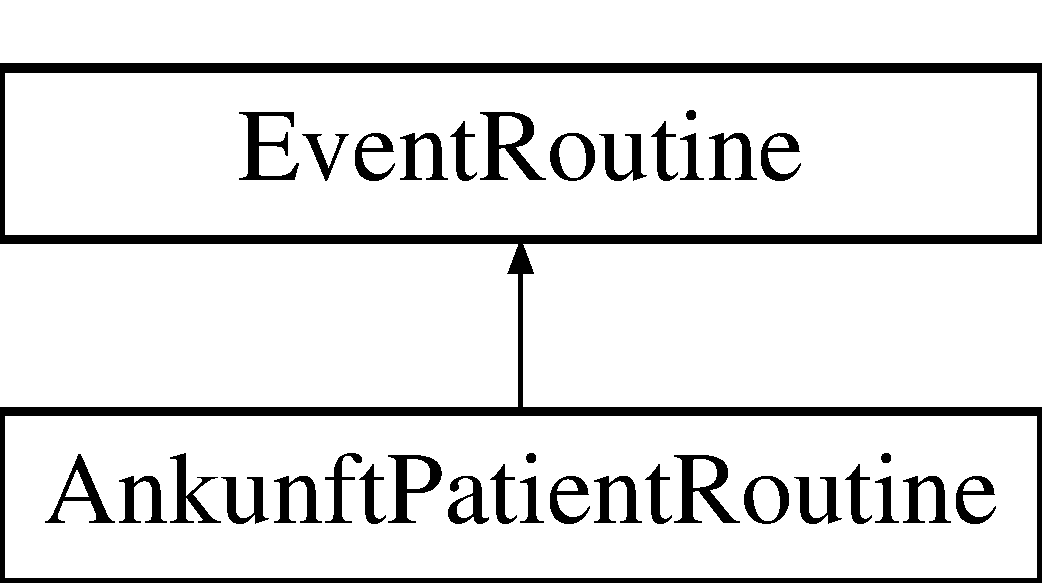
\includegraphics[height=2.000000cm]{classAnkunftPatientRoutine}
\end{center}
\end{figure}
\subsection*{Öffentliche Methoden}
\begin{DoxyCompactItemize}
\item 
\hyperlink{classAnkunftPatientRoutine_af9bd136552d3e2acd505620ca5164f58}{Ankunft\+Patient\+Routine} (\hyperlink{classNotarzt}{Notarzt} $\ast$arzt, \hyperlink{classEventList}{Event\+List} $\ast$e\+List, \hyperlink{classNotfallWarteschlange}{Notfall\+Warteschlange} $\ast$warteschlange)
\begin{DoxyCompactList}\small\item\em Konstruktor. \end{DoxyCompactList}\item 
void \hyperlink{classAnkunftPatientRoutine_a42cdf97821606ce3d4f807b685f3a70d}{execute} (\hyperlink{classEvent}{Event} $\ast$event)
\begin{DoxyCompactList}\small\item\em Spezifizierung der Zustandsänderungen. \end{DoxyCompactList}\end{DoxyCompactItemize}


\subsection{Ausführliche Beschreibung}
Routine für die Ankunft des Notarztes beim Patienten. 

Diese Routine beschreibt die Zustandsänderungen in der Notarzt-\/\+Simulation wenn der \hyperlink{classNotarzt}{Notarzt} beim Patienten ankommt. 

\subsection{Beschreibung der Konstruktoren und Destruktoren}
\index{Ankunft\+Patient\+Routine@{Ankunft\+Patient\+Routine}!Ankunft\+Patient\+Routine@{Ankunft\+Patient\+Routine}}
\index{Ankunft\+Patient\+Routine@{Ankunft\+Patient\+Routine}!Ankunft\+Patient\+Routine@{Ankunft\+Patient\+Routine}}
\subsubsection[{\texorpdfstring{Ankunft\+Patient\+Routine(\+Notarzt $\ast$arzt, Event\+List $\ast$e\+List, Notfall\+Warteschlange $\ast$warteschlange)}{AnkunftPatientRoutine(Notarzt *arzt, EventList *eList, NotfallWarteschlange *warteschlange)}}]{\setlength{\rightskip}{0pt plus 5cm}Ankunft\+Patient\+Routine\+::\+Ankunft\+Patient\+Routine (
\begin{DoxyParamCaption}
\item[{{\bf Notarzt} $\ast$}]{arzt, }
\item[{{\bf Event\+List} $\ast$}]{e\+List, }
\item[{{\bf Notfall\+Warteschlange} $\ast$}]{warteschlange}
\end{DoxyParamCaption}
)}\hypertarget{classAnkunftPatientRoutine_af9bd136552d3e2acd505620ca5164f58}{}\label{classAnkunftPatientRoutine_af9bd136552d3e2acd505620ca5164f58}


Konstruktor. 

Abhängigkeiten werden injiziert und eine spezielle \hyperlink{classEventRoutine}{Event\+Routine} mit dem Event-\/\+Typ A\+N\+K\+U\+N\+F\+\_\+\+P\+A\+T\+I\+E\+NT wird erstellt. 

\subsection{Dokumentation der Elementfunktionen}
\index{Ankunft\+Patient\+Routine@{Ankunft\+Patient\+Routine}!execute@{execute}}
\index{execute@{execute}!Ankunft\+Patient\+Routine@{Ankunft\+Patient\+Routine}}
\subsubsection[{\texorpdfstring{execute(\+Event $\ast$event)}{execute(Event *event)}}]{\setlength{\rightskip}{0pt plus 5cm}void Ankunft\+Patient\+Routine\+::execute (
\begin{DoxyParamCaption}
\item[{{\bf Event} $\ast$}]{event}
\end{DoxyParamCaption}
)\hspace{0.3cm}{\ttfamily [virtual]}}\hypertarget{classAnkunftPatientRoutine_a42cdf97821606ce3d4f807b685f3a70d}{}\label{classAnkunftPatientRoutine_a42cdf97821606ce3d4f807b685f3a70d}


Spezifizierung der Zustandsänderungen. 

Die Ankunft des Notarztes beim Patienten verändert den Zustand des Notarztes und entfernt den zugehörigen \hyperlink{classNotfall}{Notfall}, der nun behandelt wird, aus der Notfall-\/\+Warteschlange. Ein neues \hyperlink{classEvent}{Event} für das Ende der Behandlung wird der Simulation hinzugefügt, der Zeitpunkt dieses Events entsprechend berechnet. 

Implementiert \hyperlink{classEventRoutine_aede9b0fdb576a4a262ced2d7d6548c14}{Event\+Routine}.



Die Dokumentation für diese Klasse wurde erzeugt aufgrund der Dateien\+:\begin{DoxyCompactItemize}
\item 
/home/mkemp/\+Studium/\+Diskrete\+Simulation/notarzt-\/sim/source/include/Ankunft\+Patient\+Routine.\+h\item 
/home/mkemp/\+Studium/\+Diskrete\+Simulation/notarzt-\/sim/source/src/Ankunft\+Patient\+Routine.\+cpp\end{DoxyCompactItemize}

\hypertarget{classAnkunftZentraleRoutine}{}\section{Ankunft\+Zentrale\+Routine Klassenreferenz}
\label{classAnkunftZentraleRoutine}\index{Ankunft\+Zentrale\+Routine@{Ankunft\+Zentrale\+Routine}}


Routine für die Ankunft des Notarztes in der Zentrale.  




{\ttfamily \#include $<$Ankunft\+Zentrale\+Routine.\+h$>$}

Klassendiagramm für Ankunft\+Zentrale\+Routine\+:\begin{figure}[H]
\begin{center}
\leavevmode
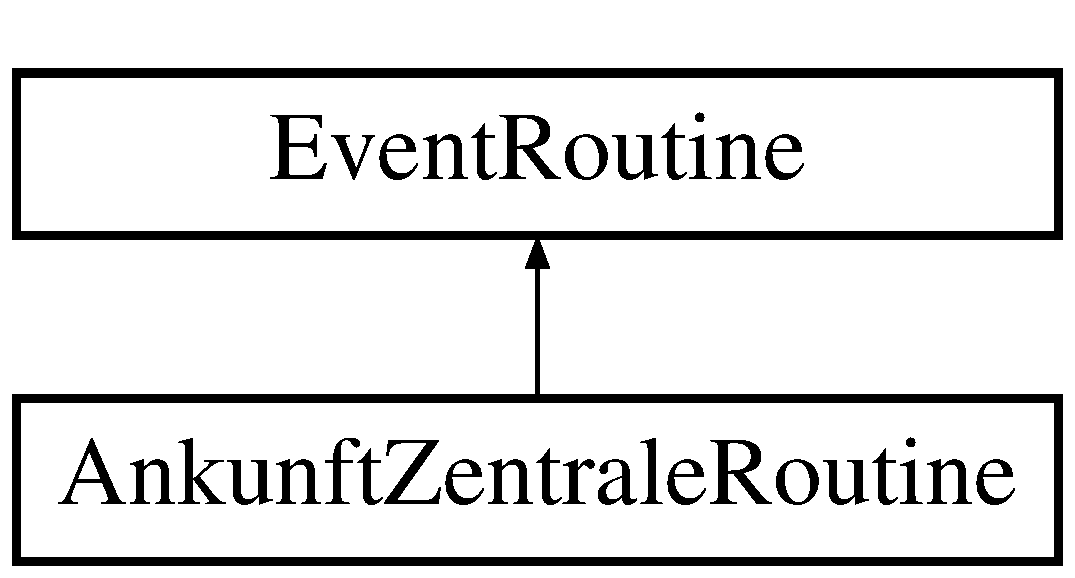
\includegraphics[height=2.000000cm]{classAnkunftZentraleRoutine}
\end{center}
\end{figure}
\subsection*{Öffentliche Methoden}
\begin{DoxyCompactItemize}
\item 
\hyperlink{classAnkunftZentraleRoutine_a04a836512c946b6486b0c27500c3f220}{Ankunft\+Zentrale\+Routine} (\hyperlink{classNotarzt}{Notarzt} $\ast$notarzt, \hyperlink{classEventList}{Event\+List} $\ast$event\+List, \hyperlink{classNotfallWarteschlange}{Notfall\+Warteschlange} $\ast$notfall\+Warteschlange)
\begin{DoxyCompactList}\small\item\em Konstruktor. \end{DoxyCompactList}\item 
void \hyperlink{classAnkunftZentraleRoutine_ab6d6422067bb87d64f4973c68c6d796a}{execute} (\hyperlink{classEvent}{Event} $\ast$event)
\begin{DoxyCompactList}\small\item\em Spezifizierung der Zustandsänderungen. \end{DoxyCompactList}\end{DoxyCompactItemize}


\subsection{Ausführliche Beschreibung}
Routine für die Ankunft des Notarztes in der Zentrale. 

Diese Routine beschreibt die Zustandsänderungen in der Notarzt-\/\+Simulation wenn der \hyperlink{classNotarzt}{Notarzt} in der Zentrale ankommt. 

\subsection{Beschreibung der Konstruktoren und Destruktoren}
\index{Ankunft\+Zentrale\+Routine@{Ankunft\+Zentrale\+Routine}!Ankunft\+Zentrale\+Routine@{Ankunft\+Zentrale\+Routine}}
\index{Ankunft\+Zentrale\+Routine@{Ankunft\+Zentrale\+Routine}!Ankunft\+Zentrale\+Routine@{Ankunft\+Zentrale\+Routine}}
\subsubsection[{\texorpdfstring{Ankunft\+Zentrale\+Routine(\+Notarzt $\ast$notarzt, Event\+List $\ast$event\+List, Notfall\+Warteschlange $\ast$notfall\+Warteschlange)}{AnkunftZentraleRoutine(Notarzt *notarzt, EventList *eventList, NotfallWarteschlange *notfallWarteschlange)}}]{\setlength{\rightskip}{0pt plus 5cm}Ankunft\+Zentrale\+Routine\+::\+Ankunft\+Zentrale\+Routine (
\begin{DoxyParamCaption}
\item[{{\bf Notarzt} $\ast$}]{notarzt, }
\item[{{\bf Event\+List} $\ast$}]{event\+List, }
\item[{{\bf Notfall\+Warteschlange} $\ast$}]{notfall\+Warteschlange}
\end{DoxyParamCaption}
)}\hypertarget{classAnkunftZentraleRoutine_a04a836512c946b6486b0c27500c3f220}{}\label{classAnkunftZentraleRoutine_a04a836512c946b6486b0c27500c3f220}


Konstruktor. 

Abhängigkeiten werden injiziert eine spezielle \hyperlink{classEventRoutine}{Event\+Routine} mit dem Event-\/\+Typ A\+N\+K\+U\+N\+F\+T\+\_\+\+Z\+E\+N\+T\+R\+A\+LE wird erstellt. 

\subsection{Dokumentation der Elementfunktionen}
\index{Ankunft\+Zentrale\+Routine@{Ankunft\+Zentrale\+Routine}!execute@{execute}}
\index{execute@{execute}!Ankunft\+Zentrale\+Routine@{Ankunft\+Zentrale\+Routine}}
\subsubsection[{\texorpdfstring{execute(\+Event $\ast$event)}{execute(Event *event)}}]{\setlength{\rightskip}{0pt plus 5cm}void Ankunft\+Zentrale\+Routine\+::execute (
\begin{DoxyParamCaption}
\item[{{\bf Event} $\ast$}]{event}
\end{DoxyParamCaption}
)\hspace{0.3cm}{\ttfamily [virtual]}}\hypertarget{classAnkunftZentraleRoutine_ab6d6422067bb87d64f4973c68c6d796a}{}\label{classAnkunftZentraleRoutine_ab6d6422067bb87d64f4973c68c6d796a}


Spezifizierung der Zustandsänderungen. 

Die Ankunft des Notarztes in der Zentrale verändert den Zustand des Notarztes auf wartend und erzeugt bei bei Bedarf ein neues \hyperlink{classEvent}{Event}. Das neue \hyperlink{classEvent}{Event} vom Typ Abfahrt\+\_\+\+Patient ist abhängig davon, ob bereits ein weiterer \hyperlink{classNotfall}{Notfall} vorliegt oder nicht. 

Implementiert \hyperlink{classEventRoutine_aede9b0fdb576a4a262ced2d7d6548c14}{Event\+Routine}.



Die Dokumentation für diese Klasse wurde erzeugt aufgrund der Dateien\+:\begin{DoxyCompactItemize}
\item 
/home/mkemp/\+Studium/\+Diskrete\+Simulation/notarzt-\/sim/source/include/Ankunft\+Zentrale\+Routine.\+h\item 
/home/mkemp/\+Studium/\+Diskrete\+Simulation/notarzt-\/sim/source/src/Ankunft\+Zentrale\+Routine.\+cpp\end{DoxyCompactItemize}

\hypertarget{classEndeBehandlungRoutine}{}\section{Ende\+Behandlung\+Routine Klassenreferenz}
\label{classEndeBehandlungRoutine}\index{Ende\+Behandlung\+Routine@{Ende\+Behandlung\+Routine}}


Routine für das Ende einer Behandlung eines Notfalls.  




{\ttfamily \#include $<$Ende\+Behandlung\+Routine.\+h$>$}

Klassendiagramm für Ende\+Behandlung\+Routine\+:\begin{figure}[H]
\begin{center}
\leavevmode
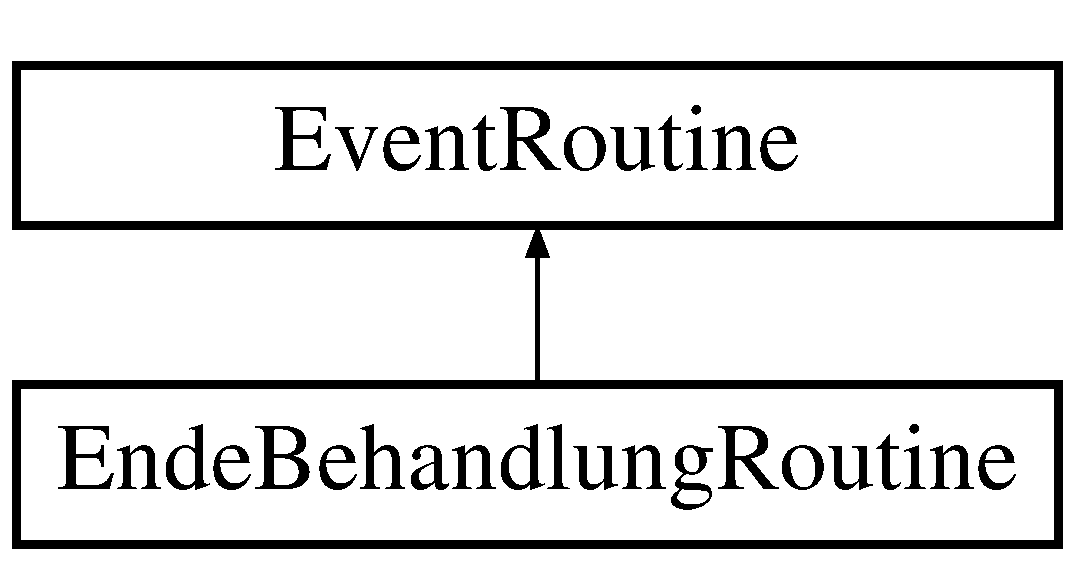
\includegraphics[height=2.000000cm]{classEndeBehandlungRoutine}
\end{center}
\end{figure}
\subsection*{Öffentliche Methoden}
\begin{DoxyCompactItemize}
\item 
\hyperlink{classEndeBehandlungRoutine_a62832ad29d885996aef9ca7f3a8ca169}{Ende\+Behandlung\+Routine} (\hyperlink{classNotarzt}{Notarzt} $\ast$notarzt, \hyperlink{classEventList}{Event\+List} $\ast$event\+List, \hyperlink{classNotfallWarteschlange}{Notfall\+Warteschlange} $\ast$notfall\+Warteschlange)
\begin{DoxyCompactList}\small\item\em Konstruktor. \end{DoxyCompactList}\item 
void \hyperlink{classEndeBehandlungRoutine_a462bdb38325bd4b5d550d4d9145e1558}{execute} (\hyperlink{classEvent}{Event} $\ast$event)
\begin{DoxyCompactList}\small\item\em Spezifizierung der Zustandsänderungen. \end{DoxyCompactList}\end{DoxyCompactItemize}


\subsection{Ausführliche Beschreibung}
Routine für das Ende einer Behandlung eines Notfalls. 

Diese Routine beschreibt die Zustandsänderungen in der Notarzt-\/\+Simulation wenn die Behandlung eines Notfalls abgeschlossen ist. 

\subsection{Beschreibung der Konstruktoren und Destruktoren}
\index{Ende\+Behandlung\+Routine@{Ende\+Behandlung\+Routine}!Ende\+Behandlung\+Routine@{Ende\+Behandlung\+Routine}}
\index{Ende\+Behandlung\+Routine@{Ende\+Behandlung\+Routine}!Ende\+Behandlung\+Routine@{Ende\+Behandlung\+Routine}}
\subsubsection[{\texorpdfstring{Ende\+Behandlung\+Routine(\+Notarzt $\ast$notarzt, Event\+List $\ast$event\+List, Notfall\+Warteschlange $\ast$notfall\+Warteschlange)}{EndeBehandlungRoutine(Notarzt *notarzt, EventList *eventList, NotfallWarteschlange *notfallWarteschlange)}}]{\setlength{\rightskip}{0pt plus 5cm}Ende\+Behandlung\+Routine\+::\+Ende\+Behandlung\+Routine (
\begin{DoxyParamCaption}
\item[{{\bf Notarzt} $\ast$}]{notarzt, }
\item[{{\bf Event\+List} $\ast$}]{event\+List, }
\item[{{\bf Notfall\+Warteschlange} $\ast$}]{notfall\+Warteschlange}
\end{DoxyParamCaption}
)}\hypertarget{classEndeBehandlungRoutine_a62832ad29d885996aef9ca7f3a8ca169}{}\label{classEndeBehandlungRoutine_a62832ad29d885996aef9ca7f3a8ca169}


Konstruktor. 

Abhängigkeiten werden injiziert und eine spezielle \hyperlink{classEventRoutine}{Event\+Routine} mit dem Event-\/\+Typ E\+N\+D\+E\+\_\+\+B\+E\+H\+A\+N\+D\+L\+U\+NG wird erstellt. 

\subsection{Dokumentation der Elementfunktionen}
\index{Ende\+Behandlung\+Routine@{Ende\+Behandlung\+Routine}!execute@{execute}}
\index{execute@{execute}!Ende\+Behandlung\+Routine@{Ende\+Behandlung\+Routine}}
\subsubsection[{\texorpdfstring{execute(\+Event $\ast$event)}{execute(Event *event)}}]{\setlength{\rightskip}{0pt plus 5cm}void Ende\+Behandlung\+Routine\+::execute (
\begin{DoxyParamCaption}
\item[{{\bf Event} $\ast$}]{event}
\end{DoxyParamCaption}
)\hspace{0.3cm}{\ttfamily [virtual]}}\hypertarget{classEndeBehandlungRoutine_a462bdb38325bd4b5d550d4d9145e1558}{}\label{classEndeBehandlungRoutine_a462bdb38325bd4b5d550d4d9145e1558}


Spezifizierung der Zustandsänderungen. 

Das Ende der Behandlung eines Notfalls bzw. Patienten verändert den Zustand des Notarztes. Dabei muss zuerst entschieden werden, ob der \hyperlink{classNotarzt}{Notarzt} gleich zu einem weiterem \hyperlink{classNotfall}{Notfall} fahren muss oder zurück in die Zentrale fährt. Einentsprechendes \hyperlink{classEvent}{Event} entweder vom Typ A\+B\+F\+A\+H\+R\+T\+\_\+\+Z\+U\+\_\+\+P\+A\+T\+I\+E\+NT oder A\+B\+F\+A\+H\+R\+T\+\_\+\+Z\+U\+\_\+\+Z\+E\+N\+T\+R\+A\+LE wird erstellt. Dieses abhängige \hyperlink{classEvent}{Event} (abhängig von E\+N\+D\+E\+\_\+\+B\+E\+H\+A\+N\+D\+L\+U\+NG) bekommt als Zeitpunkt der Erscheinung den selben Zeitpunkt wie das \hyperlink{classEvent}{Event} vom Typ E\+N\+D\+E\+\_\+\+B\+E\+H\+A\+N\+D\+L\+U\+NG, welches diese Routine ausgelöst hat. Es passiert also in der Simulation augenblicklich ohne Zeitverzögerung. 

Implementiert \hyperlink{classEventRoutine_aede9b0fdb576a4a262ced2d7d6548c14}{Event\+Routine}.



Die Dokumentation für diese Klasse wurde erzeugt aufgrund der Dateien\+:\begin{DoxyCompactItemize}
\item 
/home/mkemp/\+Studium/\+Diskrete\+Simulation/notarzt-\/sim/source/include/Ende\+Behandlung\+Routine.\+h\item 
/home/mkemp/\+Studium/\+Diskrete\+Simulation/notarzt-\/sim/source/src/Ende\+Behandlung\+Routine.\+cpp\end{DoxyCompactItemize}

\hypertarget{classEndRoutine}{}\section{End\+Routine Klassenreferenz}
\label{classEndRoutine}\index{End\+Routine@{End\+Routine}}
Klassendiagramm für End\+Routine\+:\begin{figure}[H]
\begin{center}
\leavevmode
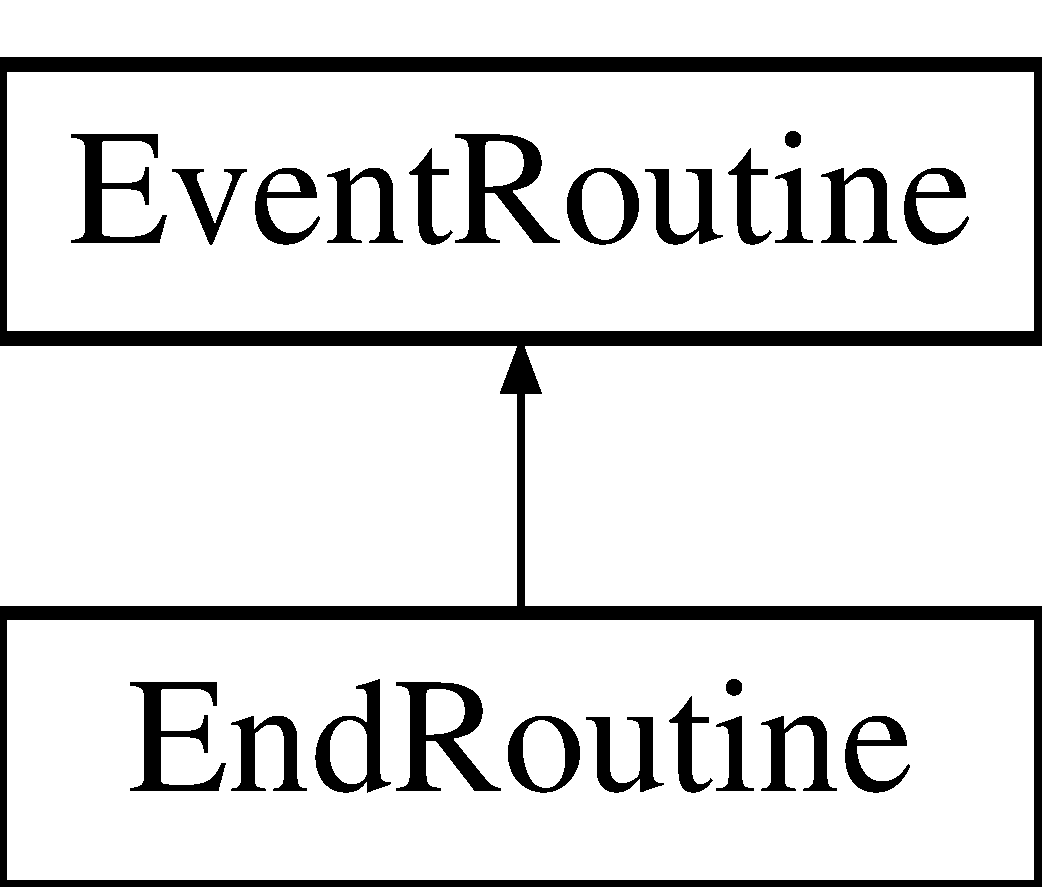
\includegraphics[height=2.000000cm]{classEndRoutine}
\end{center}
\end{figure}
\subsection*{Öffentliche Methoden}
\begin{DoxyCompactItemize}
\item 
{\bfseries End\+Routine} (Event\+Type t)\hypertarget{classEndRoutine_af6bdd3a9c499fcb62ebdd24758763eb8}{}\label{classEndRoutine_af6bdd3a9c499fcb62ebdd24758763eb8}

\item 
void {\bfseries execute} (\hyperlink{classEvent}{Event} $\ast$event)\hypertarget{classEndRoutine_a147e1143dfec1d3fb4a58d3a6efd6641}{}\label{classEndRoutine_a147e1143dfec1d3fb4a58d3a6efd6641}

\end{DoxyCompactItemize}


Die Dokumentation für diese Klasse wurde erzeugt aufgrund der Dateien\+:\begin{DoxyCompactItemize}
\item 
/home/mkemp/\+Studium/\+Diskrete\+Simulation/notarzt-\/sim/source/include/End\+Routine.\+h\item 
/home/mkemp/\+Studium/\+Diskrete\+Simulation/notarzt-\/sim/source/src/End\+Routine.\+cpp\end{DoxyCompactItemize}

\hypertarget{classEvent}{}\section{Event Klassenreferenz}
\label{classEvent}\index{Event@{Event}}


{\ttfamily \#include $<$Event.\+h$>$}

\subsection*{Öffentliche Methoden}
\begin{DoxyCompactItemize}
\item 
\hyperlink{classEvent_ac7422ad6f411427e4d51cde6bcc51572}{Event} (int execution\+Time, Event\+Type type)
\item 
int {\bfseries get\+Execution\+Time} ()\hypertarget{classEvent_aa96b4d982f3330662aa94a03c2aa9df3}{}\label{classEvent_aa96b4d982f3330662aa94a03c2aa9df3}

\item 
Event\+Type {\bfseries get\+Type} ()\hypertarget{classEvent_aceb1ddcf030da7877ab5c4bf38afb1dc}{}\label{classEvent_aceb1ddcf030da7877ab5c4bf38afb1dc}

\end{DoxyCompactItemize}


\subsection{Ausführliche Beschreibung}
Implementierung eines allgemeinen Ereignises im Rahmen der diskreten, ereignisgesteureten Simulation. 

\subsection{Beschreibung der Konstruktoren und Destruktoren}
\index{Event@{Event}!Event@{Event}}
\index{Event@{Event}!Event@{Event}}
\subsubsection[{\texorpdfstring{Event(int execution\+Time, Event\+Type type)}{Event(int executionTime, EventType type)}}]{\setlength{\rightskip}{0pt plus 5cm}Event\+::\+Event (
\begin{DoxyParamCaption}
\item[{int}]{exe\+Time, }
\item[{Event\+Type}]{t}
\end{DoxyParamCaption}
)}\hypertarget{classEvent_ac7422ad6f411427e4d51cde6bcc51572}{}\label{classEvent_ac7422ad6f411427e4d51cde6bcc51572}
Implementierung eines allgemeinen Ereignises im Rahmen der diskreten, ereignisgesteureten Simulation. 

Die Dokumentation für diese Klasse wurde erzeugt aufgrund der Dateien\+:\begin{DoxyCompactItemize}
\item 
/home/mkemp/\+Studium/\+Diskrete\+Simulation/notarzt-\/sim/source/include/Event.\+h\item 
/home/mkemp/\+Studium/\+Diskrete\+Simulation/notarzt-\/sim/source/src/Event.\+cpp\end{DoxyCompactItemize}

\hypertarget{classEventList}{}\section{Event\+List Klassenreferenz}
\label{classEventList}\index{Event\+List@{Event\+List}}
\subsection*{Öffentliche Methoden}
\begin{DoxyCompactItemize}
\item 
\hyperlink{classEventList_afb3f0b055c2b7c5431cfe234ffcda269}{Event\+List} ()
\item 
\hyperlink{classEvent}{Event} $\ast$ {\bfseries pop\+Event} ()\hypertarget{classEventList_a0a14cce1690774fa3c88a694bc4f2572}{}\label{classEventList_a0a14cce1690774fa3c88a694bc4f2572}

\item 
\hyperlink{classEvent}{Event} $\ast$ {\bfseries get\+Next\+Event} ()\hypertarget{classEventList_aa426ac93e711b567b66f7ba3c51cb2bd}{}\label{classEventList_aa426ac93e711b567b66f7ba3c51cb2bd}

\item 
int {\bfseries remove\+Event\+By\+Type} (Event\+Type type)\hypertarget{classEventList_a3bd963a8a43cc5efcbe0059e58425985}{}\label{classEventList_a3bd963a8a43cc5efcbe0059e58425985}

\item 
void {\bfseries add\+Event} (\hyperlink{classEvent}{Event} $\ast$event)\hypertarget{classEventList_ab17b4c5ef72e741876a5563a5a281d74}{}\label{classEventList_ab17b4c5ef72e741876a5563a5a281d74}

\item 
void {\bfseries print\+List} ()\hypertarget{classEventList_a7e32e3d4bc10adb837048937a21bfb6b}{}\label{classEventList_a7e32e3d4bc10adb837048937a21bfb6b}

\end{DoxyCompactItemize}


\subsection{Beschreibung der Konstruktoren und Destruktoren}
\index{Event\+List@{Event\+List}!Event\+List@{Event\+List}}
\index{Event\+List@{Event\+List}!Event\+List@{Event\+List}}
\subsubsection[{\texorpdfstring{Event\+List()}{EventList()}}]{\setlength{\rightskip}{0pt plus 5cm}Event\+List\+::\+Event\+List (
\begin{DoxyParamCaption}
{}
\end{DoxyParamCaption}
)}\hypertarget{classEventList_afb3f0b055c2b7c5431cfe234ffcda269}{}\label{classEventList_afb3f0b055c2b7c5431cfe234ffcda269}
Ereignisliste für die diskrete, eventgesteruerte Simulation. 

Die Dokumentation für diese Klasse wurde erzeugt aufgrund der Dateien\+:\begin{DoxyCompactItemize}
\item 
/home/mkemp/\+Studium/\+Diskrete\+Simulation/notarzt-\/sim/source/include/Event\+List.\+h\item 
/home/mkemp/\+Studium/\+Diskrete\+Simulation/notarzt-\/sim/source/src/Event\+List.\+cpp\end{DoxyCompactItemize}

\hypertarget{classEventRoutine}{}\section{Event\+Routine Klassenreferenz}
\label{classEventRoutine}\index{Event\+Routine@{Event\+Routine}}


Abstrakte Erignis-\/\+Routine.  




{\ttfamily \#include $<$Event\+Routine.\+h$>$}

Klassendiagramm für Event\+Routine\+:\begin{figure}[H]
\begin{center}
\leavevmode
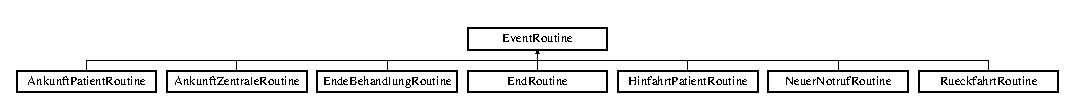
\includegraphics[height=1.012658cm]{classEventRoutine}
\end{center}
\end{figure}
\subsection*{Öffentliche Methoden}
\begin{DoxyCompactItemize}
\item 
\hyperlink{classEventRoutine_acd33ef6e5acc459719005276cc9c55e9}{Event\+Routine} (Event\+Type type)
\begin{DoxyCompactList}\small\item\em Konstruktor. \end{DoxyCompactList}\item 
virtual void \hyperlink{classEventRoutine_aede9b0fdb576a4a262ced2d7d6548c14}{execute} (\hyperlink{classEvent}{Event} $\ast$event)=0
\begin{DoxyCompactList}\small\item\em Funktionssignatur Ausführung einer Routine. \end{DoxyCompactList}\item 
Event\+Type \hyperlink{classEventRoutine_afcaf1409efcd2b6572b54c7a6fc02428}{get\+Type} ()
\begin{DoxyCompactList}\small\item\em Liefert Ereignistyp. \end{DoxyCompactList}\end{DoxyCompactItemize}


\subsection{Ausführliche Beschreibung}
Abstrakte Erignis-\/\+Routine. 

Abstrakte Klasse für die minimale Definition einer Ereignisroutine in einer diskreten, eventgesteuerten Simulation. 

\subsection{Beschreibung der Konstruktoren und Destruktoren}
\index{Event\+Routine@{Event\+Routine}!Event\+Routine@{Event\+Routine}}
\index{Event\+Routine@{Event\+Routine}!Event\+Routine@{Event\+Routine}}
\subsubsection[{\texorpdfstring{Event\+Routine(\+Event\+Type type)}{EventRoutine(EventType type)}}]{\setlength{\rightskip}{0pt plus 5cm}Event\+Routine\+::\+Event\+Routine (
\begin{DoxyParamCaption}
\item[{Event\+Type}]{type}
\end{DoxyParamCaption}
)}\hypertarget{classEventRoutine_acd33ef6e5acc459719005276cc9c55e9}{}\label{classEventRoutine_acd33ef6e5acc459719005276cc9c55e9}


Konstruktor. 

Eine Routine besitzt immer einen spezifischen Typ, der von der Art der Simulation abhängig ist. Dieser Typ ermöglich der Simulationsschleife, die passende Routine zu einem \hyperlink{classEvent}{Event} zu finden. 

\subsection{Dokumentation der Elementfunktionen}
\index{Event\+Routine@{Event\+Routine}!execute@{execute}}
\index{execute@{execute}!Event\+Routine@{Event\+Routine}}
\subsubsection[{\texorpdfstring{execute(\+Event $\ast$event)=0}{execute(Event *event)=0}}]{\setlength{\rightskip}{0pt plus 5cm}virtual void Event\+Routine\+::execute (
\begin{DoxyParamCaption}
\item[{{\bf Event} $\ast$}]{event}
\end{DoxyParamCaption}
)\hspace{0.3cm}{\ttfamily [pure virtual]}}\hypertarget{classEventRoutine_aede9b0fdb576a4a262ced2d7d6548c14}{}\label{classEventRoutine_aede9b0fdb576a4a262ced2d7d6548c14}


Funktionssignatur Ausführung einer Routine. 

Abstrakte Funktion, die die Erwartungshaltung an alle implementierten Ereignisroutinen definiert. Das ermöglicht eine allgemeine Definition der Simulationsschleife ohne dass spezielle Wissen über die implementierten Ereignisroutinen notwendig ist.

Muss von jeder spezialisierenden Klasse implementiert werden 

Implementiert in \hyperlink{classHinfahrtPatientRoutine_a95ee9981032536e15cad4bbe0fcb6903}{Hinfahrt\+Patient\+Routine}, \hyperlink{classNeuerNotrufRoutine_af2d883cecce5e012c9332c933c1cb10f}{Neuer\+Notruf\+Routine}, \hyperlink{classEndeBehandlungRoutine_a462bdb38325bd4b5d550d4d9145e1558}{Ende\+Behandlung\+Routine}, \hyperlink{classAnkunftPatientRoutine_a42cdf97821606ce3d4f807b685f3a70d}{Ankunft\+Patient\+Routine}, \hyperlink{classRueckfahrtRoutine_a7eec059994f3c958696697df05cfefe9}{Rueckfahrt\+Routine}, \hyperlink{classAnkunftZentraleRoutine_ab6d6422067bb87d64f4973c68c6d796a}{Ankunft\+Zentrale\+Routine} und \hyperlink{classEndRoutine_a147e1143dfec1d3fb4a58d3a6efd6641}{End\+Routine}.

\index{Event\+Routine@{Event\+Routine}!get\+Type@{get\+Type}}
\index{get\+Type@{get\+Type}!Event\+Routine@{Event\+Routine}}
\subsubsection[{\texorpdfstring{get\+Type()}{getType()}}]{\setlength{\rightskip}{0pt plus 5cm}Event\+Type Event\+Routine\+::get\+Type (
\begin{DoxyParamCaption}
{}
\end{DoxyParamCaption}
)}\hypertarget{classEventRoutine_afcaf1409efcd2b6572b54c7a6fc02428}{}\label{classEventRoutine_afcaf1409efcd2b6572b54c7a6fc02428}


Liefert Ereignistyp. 

Fertig implementierte Funtkion zur Rückgabe des Eriegnistyps. 

Die Dokumentation für diese Klasse wurde erzeugt aufgrund der Dateien\+:\begin{DoxyCompactItemize}
\item 
/home/mkemp/\+Studium/\+Diskrete\+Simulation/notarzt-\/sim/source/include/Event\+Routine.\+h\item 
/home/mkemp/\+Studium/\+Diskrete\+Simulation/notarzt-\/sim/source/src/Event\+Routine.\+cpp\end{DoxyCompactItemize}

\hypertarget{classHinfahrtPatientRoutine}{}\section{Hinfahrt\+Patient\+Routine Klassenreferenz}
\label{classHinfahrtPatientRoutine}\index{Hinfahrt\+Patient\+Routine@{Hinfahrt\+Patient\+Routine}}
Klassendiagramm für Hinfahrt\+Patient\+Routine\+:\begin{figure}[H]
\begin{center}
\leavevmode
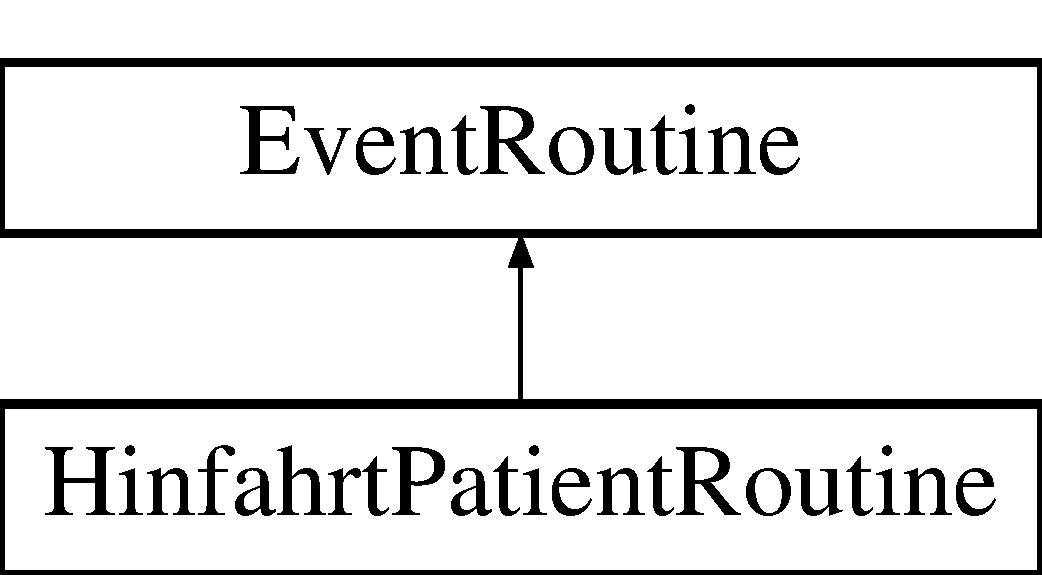
\includegraphics[height=2.000000cm]{classHinfahrtPatientRoutine}
\end{center}
\end{figure}
\subsection*{Öffentliche Methoden}
\begin{DoxyCompactItemize}
\item 
{\bfseries Hinfahrt\+Patient\+Routine} (\hyperlink{classNotarzt}{Notarzt} $\ast$notarzt, \hyperlink{classEventList}{Event\+List} $\ast$event\+List, \hyperlink{classNotfallWarteschlange}{Notfall\+Warteschlange} $\ast$notfall\+Warteschlange, \hyperlink{classZufall}{Zufall} $\ast$random\+Generator)\hypertarget{classHinfahrtPatientRoutine_aef87b22e6bb463ec319534f2e33ba8be}{}\label{classHinfahrtPatientRoutine_aef87b22e6bb463ec319534f2e33ba8be}

\item 
void {\bfseries execute} (\hyperlink{classEvent}{Event} $\ast$event)\hypertarget{classHinfahrtPatientRoutine_a95ee9981032536e15cad4bbe0fcb6903}{}\label{classHinfahrtPatientRoutine_a95ee9981032536e15cad4bbe0fcb6903}

\end{DoxyCompactItemize}


Die Dokumentation für diese Klasse wurde erzeugt aufgrund der Dateien\+:\begin{DoxyCompactItemize}
\item 
/home/mkemp/\+Studium/\+Diskrete\+Simulation/notarzt-\/sim/source/include/Hinfahrt\+Patient\+Routine.\+h\item 
/home/mkemp/\+Studium/\+Diskrete\+Simulation/notarzt-\/sim/source/src/Hinfahrt\+Patient\+Routine.\+cpp\end{DoxyCompactItemize}

\hypertarget{classNeuerNotrufRoutine}{}\section{Neuer\+Notruf\+Routine Klassenreferenz}
\label{classNeuerNotrufRoutine}\index{Neuer\+Notruf\+Routine@{Neuer\+Notruf\+Routine}}
Klassendiagramm für Neuer\+Notruf\+Routine\+:\begin{figure}[H]
\begin{center}
\leavevmode
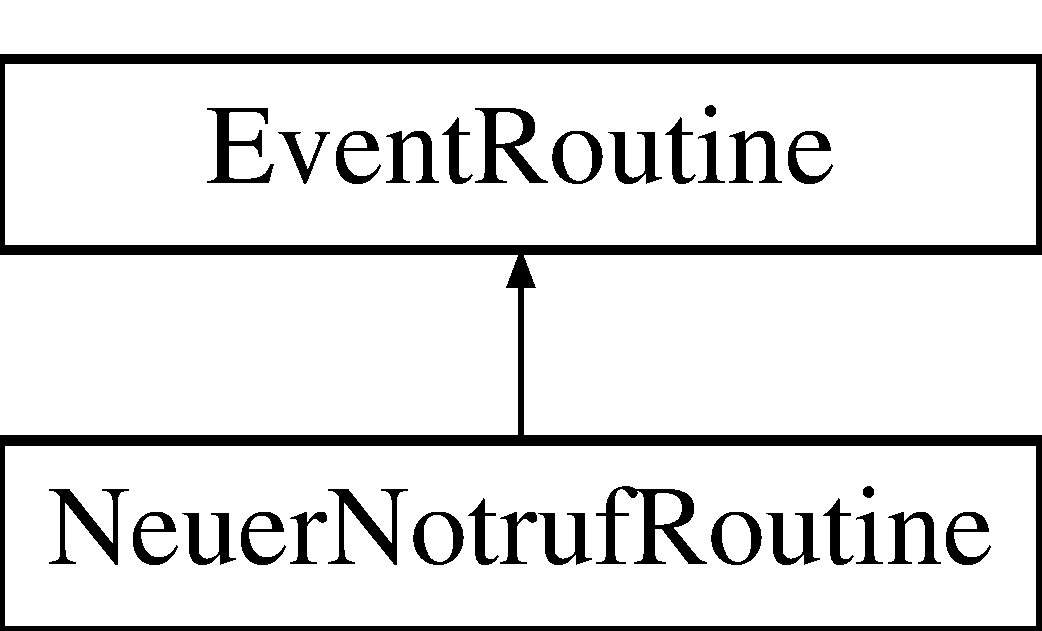
\includegraphics[height=2.000000cm]{classNeuerNotrufRoutine}
\end{center}
\end{figure}
\subsection*{Öffentliche Methoden}
\begin{DoxyCompactItemize}
\item 
{\bfseries Neuer\+Notruf\+Routine} (\hyperlink{classNotfallWarteschlange}{Notfall\+Warteschlange} $\ast$n, \hyperlink{classNotarzt}{Notarzt} $\ast$arzt, \hyperlink{classEventList}{Event\+List} $\ast$e\+List, \hyperlink{classZufall}{Zufall} $\ast$random\+Gen)\hypertarget{classNeuerNotrufRoutine_a80f789ceb242c142833658db7f28a686}{}\label{classNeuerNotrufRoutine_a80f789ceb242c142833658db7f28a686}

\item 
void {\bfseries execute} (\hyperlink{classEvent}{Event} $\ast$event)\hypertarget{classNeuerNotrufRoutine_af2d883cecce5e012c9332c933c1cb10f}{}\label{classNeuerNotrufRoutine_af2d883cecce5e012c9332c933c1cb10f}

\end{DoxyCompactItemize}


Die Dokumentation für diese Klasse wurde erzeugt aufgrund der Dateien\+:\begin{DoxyCompactItemize}
\item 
/home/mkemp/\+Studium/\+Diskrete\+Simulation/notarzt-\/sim/source/include/Neuer\+Notruf\+Routine.\+h\item 
/home/mkemp/\+Studium/\+Diskrete\+Simulation/notarzt-\/sim/source/src/Neuer\+Notruf\+Routine.\+cpp\end{DoxyCompactItemize}

\hypertarget{classNotarzt}{}\section{Notarzt Klassenreferenz}
\label{classNotarzt}\index{Notarzt@{Notarzt}}


Repräsentiert einen \hyperlink{classNotarzt}{Notarzt}.  




{\ttfamily \#include $<$Notarzt.\+h$>$}

Klassendiagramm für Notarzt\+:\begin{figure}[H]
\begin{center}
\leavevmode
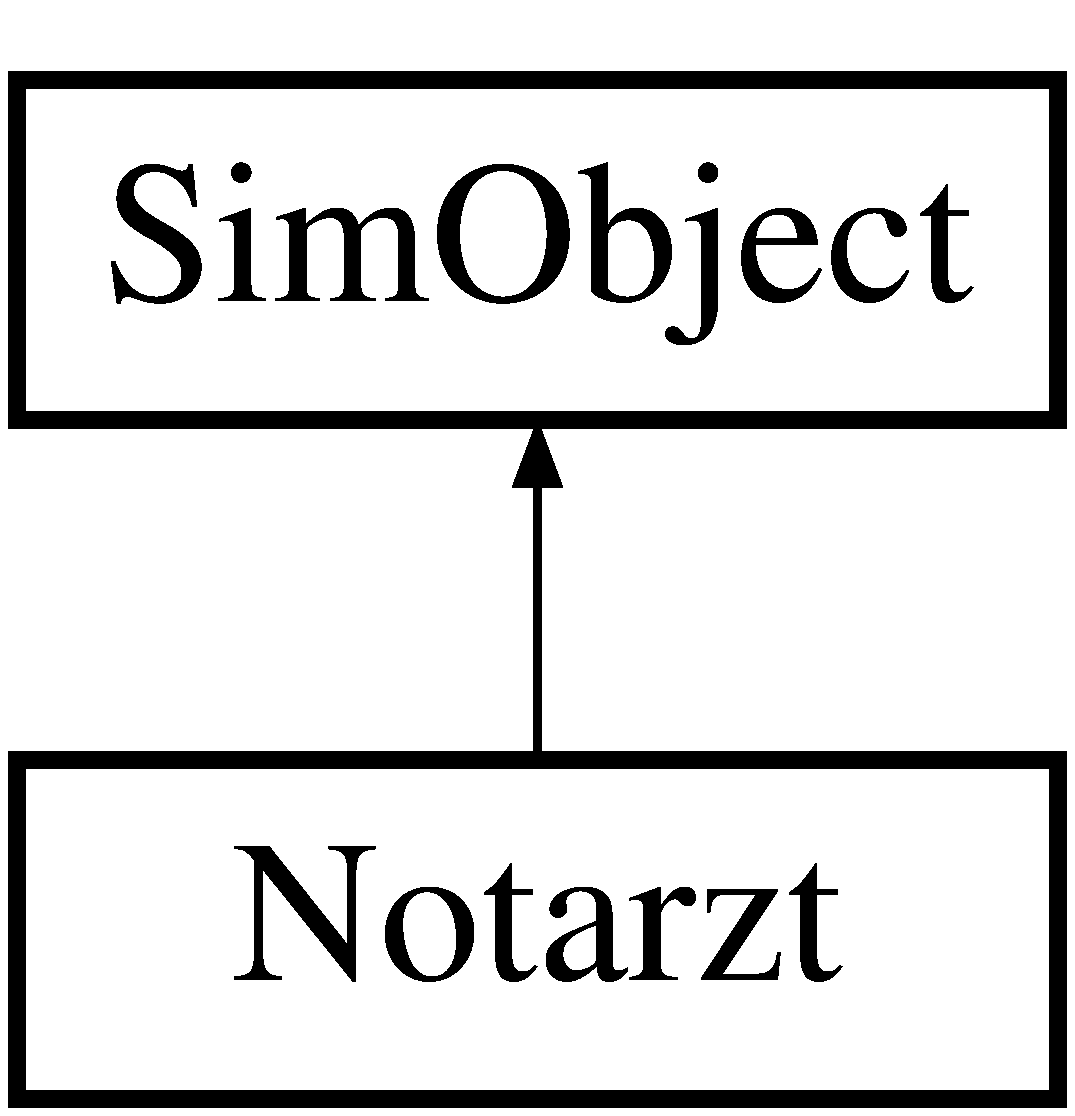
\includegraphics[height=2.000000cm]{classNotarzt}
\end{center}
\end{figure}
\subsection*{Öffentliche Methoden}
\begin{DoxyCompactItemize}
\item 
\hyperlink{classNotarzt_af90cdea1ef049791cf09cd6d1e9f8399}{Notarzt} (Notarzt\+States state, int place)
\begin{DoxyCompactList}\small\item\em Konstruktor. \end{DoxyCompactList}\item 
int {\bfseries get\+Timestamp} ()\hypertarget{classNotarzt_af94182cd4fc47929260c9ce3e129028f}{}\label{classNotarzt_af94182cd4fc47929260c9ce3e129028f}

\item 
Notarzt\+States {\bfseries get\+Notarzt\+State} ()\hypertarget{classNotarzt_a460b020d5f78bf43de6d82b30315bc68}{}\label{classNotarzt_a460b020d5f78bf43de6d82b30315bc68}

\item 
int {\bfseries get\+Notarzt\+Place} ()\hypertarget{classNotarzt_a066e840824b26d97d7e02f5eb697bf33}{}\label{classNotarzt_a066e840824b26d97d7e02f5eb697bf33}

\item 
void {\bfseries set\+Timestamp} (int new\+Timestamp)\hypertarget{classNotarzt_a2443bb2d3a8fad6ad868db80d93add93}{}\label{classNotarzt_a2443bb2d3a8fad6ad868db80d93add93}

\item 
void {\bfseries set\+Notarzt\+State} (Notarzt\+States new\+State)\hypertarget{classNotarzt_a08bfaf5815206e487ff29d87f0e9ab0c}{}\label{classNotarzt_a08bfaf5815206e487ff29d87f0e9ab0c}

\item 
void {\bfseries set\+Notarzt\+Place} (int new\+Place)\hypertarget{classNotarzt_a3ccdfae8cbaebbe4d0ff049f05e78016}{}\label{classNotarzt_a3ccdfae8cbaebbe4d0ff049f05e78016}

\item 
void \hyperlink{classNotarzt_a938d1d749b2741f3dc426e24a437c43c}{get\+State} ()
\begin{DoxyCompactList}\small\item\em Funktionssignatur für das Abspeichern des Objektes. \end{DoxyCompactList}\end{DoxyCompactItemize}


\subsection{Ausführliche Beschreibung}
Repräsentiert einen \hyperlink{classNotarzt}{Notarzt}. 

Klasse für die Erstellung von Notarzt-\/\+Objekten, die in der Notarzt-\/\+Simulation verwendet werden können. Der \hyperlink{classNotarzt}{Notarzt} besitzt keine eigen Logik sondern repräsentiert immer nur einen bestimmten Zustand des Notarztes in der Notarzt-\/\+Simulation. 

\subsection{Beschreibung der Konstruktoren und Destruktoren}
\index{Notarzt@{Notarzt}!Notarzt@{Notarzt}}
\index{Notarzt@{Notarzt}!Notarzt@{Notarzt}}
\subsubsection[{\texorpdfstring{Notarzt(\+Notarzt\+States state, int place)}{Notarzt(NotarztStates state, int place)}}]{\setlength{\rightskip}{0pt plus 5cm}Notarzt\+::\+Notarzt (
\begin{DoxyParamCaption}
\item[{Notarzt\+States}]{state, }
\item[{int}]{place}
\end{DoxyParamCaption}
)}\hypertarget{classNotarzt_af90cdea1ef049791cf09cd6d1e9f8399}{}\label{classNotarzt_af90cdea1ef049791cf09cd6d1e9f8399}


Konstruktor. 

Mit den gegebene Parametern wird der Anfangszustand des Notarztes in der Notarzt-\/\+Simulation defniert. Timestamp wird initial immer auf 0 gesetzt. 

\subsection{Dokumentation der Elementfunktionen}
\index{Notarzt@{Notarzt}!get\+State@{get\+State}}
\index{get\+State@{get\+State}!Notarzt@{Notarzt}}
\subsubsection[{\texorpdfstring{get\+State()}{getState()}}]{\setlength{\rightskip}{0pt plus 5cm}void Notarzt\+::get\+State (
\begin{DoxyParamCaption}
{}
\end{DoxyParamCaption}
)\hspace{0.3cm}{\ttfamily [virtual]}}\hypertarget{classNotarzt_a938d1d749b2741f3dc426e24a437c43c}{}\label{classNotarzt_a938d1d749b2741f3dc426e24a437c43c}


Funktionssignatur für das Abspeichern des Objektes. 

Diese Schnittstelle stellt die minimale Erwartunhshaltung an Zustands-\/\+Objekten innerhalb einer Simulation dar. Sie muss foglich von jedem speziellem Zustands-\/\+Objekt implementiert werden. Diese Funktion speichert den aktuellen Zustand des Objektes.

T\+O\+DO Wird in der aktuellen Notarzt-\/\+Implementierung nicht verwendet. Die aktuelle Architektur lässt keine allgemeien Speicherung von Sim\+Objekten zu. 

Implementiert \hyperlink{classSimObject_a3100e6db6c86456b79351c7e6a62ec65}{Sim\+Object}.



Die Dokumentation für diese Klasse wurde erzeugt aufgrund der Dateien\+:\begin{DoxyCompactItemize}
\item 
/home/mkemp/\+Studium/\+Diskrete\+Simulation/notarzt-\/sim/source/include/Notarzt.\+h\item 
/home/mkemp/\+Studium/\+Diskrete\+Simulation/notarzt-\/sim/source/src/Notarzt.\+cpp\end{DoxyCompactItemize}

\hypertarget{classNotfall}{}\section{Notfall Klassenreferenz}
\label{classNotfall}\index{Notfall@{Notfall}}
Klassendiagramm für Notfall\+:\begin{figure}[H]
\begin{center}
\leavevmode
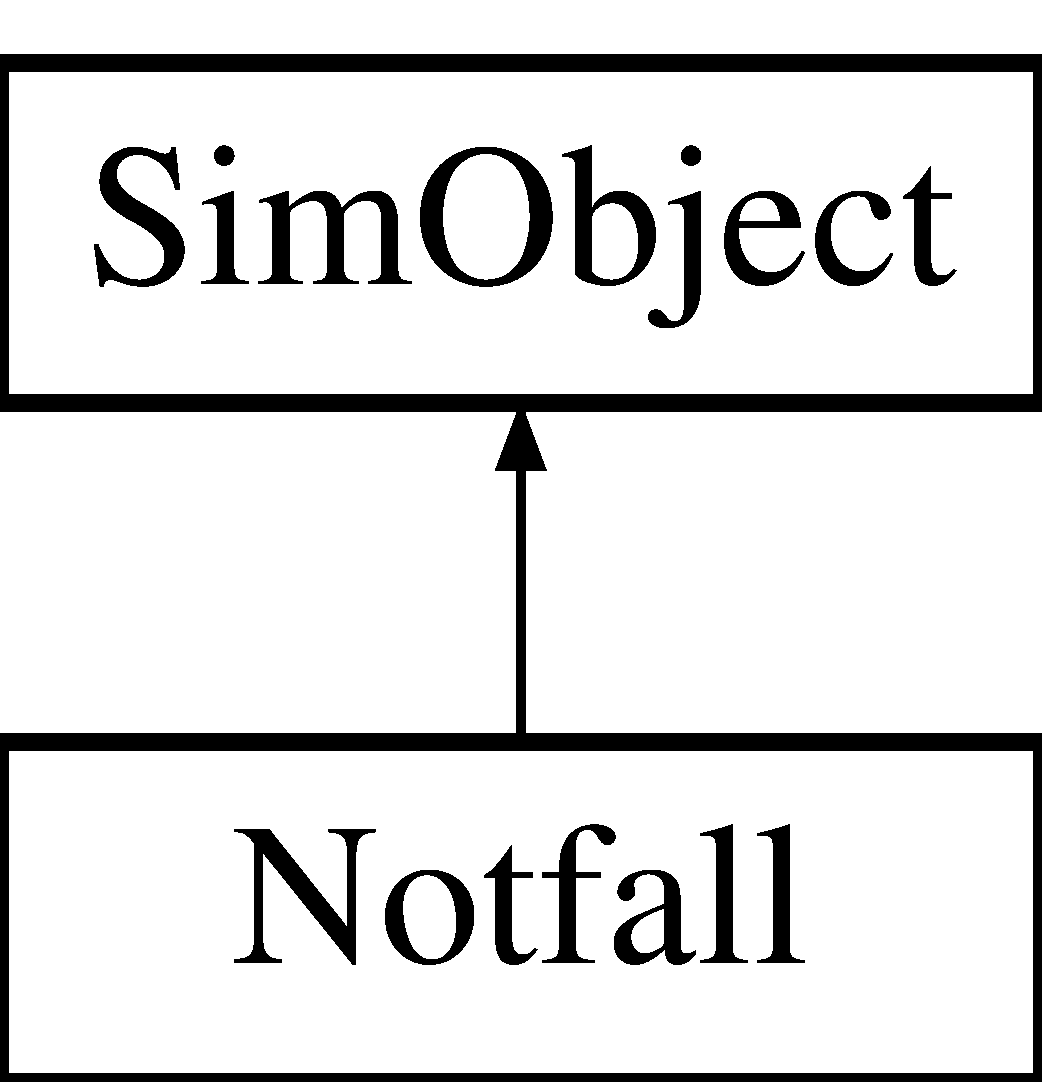
\includegraphics[height=2.000000cm]{classNotfall}
\end{center}
\end{figure}
\subsection*{Öffentliche Methoden}
\begin{DoxyCompactItemize}
\item 
{\bfseries Notfall} (int call\+Time, int prio, int treatment\+Duration, int place)\hypertarget{classNotfall_a7542c732e9bf644347982d4318b00f6e}{}\label{classNotfall_a7542c732e9bf644347982d4318b00f6e}

\item 
int {\bfseries is\+Urgent} ()\hypertarget{classNotfall_aaa4a4ffbf29b6a9bde87e89c5e182171}{}\label{classNotfall_aaa4a4ffbf29b6a9bde87e89c5e182171}

\item 
int {\bfseries get\+Call\+Time} ()\hypertarget{classNotfall_a020b9affed3c31a2de1ca25e186c14f6}{}\label{classNotfall_a020b9affed3c31a2de1ca25e186c14f6}

\item 
int {\bfseries get\+Treatment\+Duration} ()\hypertarget{classNotfall_ac7fc1ecdc2f4f5a599c48f1fc459ff33}{}\label{classNotfall_ac7fc1ecdc2f4f5a599c48f1fc459ff33}

\item 
int {\bfseries get\+Place} ()\hypertarget{classNotfall_a771c31393b277fc9d6ff72795fd9369d}{}\label{classNotfall_a771c31393b277fc9d6ff72795fd9369d}

\item 
void {\bfseries get\+State} ()\hypertarget{classNotfall_a3c65c33128d0c504f22bbefa301a0c95}{}\label{classNotfall_a3c65c33128d0c504f22bbefa301a0c95}

\end{DoxyCompactItemize}


Die Dokumentation für diese Klasse wurde erzeugt aufgrund der Dateien\+:\begin{DoxyCompactItemize}
\item 
/home/mkemp/\+Studium/\+Diskrete\+Simulation/notarzt-\/sim/source/include/Notfall.\+h\item 
/home/mkemp/\+Studium/\+Diskrete\+Simulation/notarzt-\/sim/source/src/Notfall.\+cpp\end{DoxyCompactItemize}

\hypertarget{classNotfallWarteschlange}{}\section{Notfall\+Warteschlange Klassenreferenz}
\label{classNotfallWarteschlange}\index{Notfall\+Warteschlange@{Notfall\+Warteschlange}}
\subsection*{Öffentliche Methoden}
\begin{DoxyCompactItemize}
\item 
{\bfseries Notfall\+Warteschlange} (\hyperlink{classStateStorage}{State\+Storage} $\ast$storage)\hypertarget{classNotfallWarteschlange_a6044cf77e4e6485aa182c03d03da7cd3}{}\label{classNotfallWarteschlange_a6044cf77e4e6485aa182c03d03da7cd3}

\item 
void {\bfseries add} (\hyperlink{classNotfall}{Notfall} $\ast$notfall)\hypertarget{classNotfallWarteschlange_adbe91265e4e4fa6b075714aaa6287fc6}{}\label{classNotfallWarteschlange_adbe91265e4e4fa6b075714aaa6287fc6}

\item 
\hyperlink{classNotfall}{Notfall} $\ast$ {\bfseries pop} ()\hypertarget{classNotfallWarteschlange_af941293bb468dccf5283bdba4d3ad664}{}\label{classNotfallWarteschlange_af941293bb468dccf5283bdba4d3ad664}

\item 
\hyperlink{classNotfall}{Notfall} $\ast$ {\bfseries front} ()\hypertarget{classNotfallWarteschlange_ab541fb2019e971af7fb45b995c9c8418}{}\label{classNotfallWarteschlange_ab541fb2019e971af7fb45b995c9c8418}

\item 
void {\bfseries print\+List} ()\hypertarget{classNotfallWarteschlange_aab9cd1910a42b4c6a563daec7f49cddd}{}\label{classNotfallWarteschlange_aab9cd1910a42b4c6a563daec7f49cddd}

\end{DoxyCompactItemize}


Die Dokumentation für diese Klasse wurde erzeugt aufgrund der Dateien\+:\begin{DoxyCompactItemize}
\item 
/home/mkemp/\+Studium/\+Diskrete\+Simulation/notarzt-\/sim/source/include/Notfall\+Warteschlange.\+h\item 
/home/mkemp/\+Studium/\+Diskrete\+Simulation/notarzt-\/sim/source/src/Notfall\+Warteschlange.\+cpp\end{DoxyCompactItemize}

\hypertarget{classRueckfahrtRoutine}{}\section{Rueckfahrt\+Routine Klassenreferenz}
\label{classRueckfahrtRoutine}\index{Rueckfahrt\+Routine@{Rueckfahrt\+Routine}}


Routine für die Rückfahrt zur Zentrale.  




{\ttfamily \#include $<$Rueckfahrt\+Routine.\+h$>$}

Klassendiagramm für Rueckfahrt\+Routine\+:\begin{figure}[H]
\begin{center}
\leavevmode
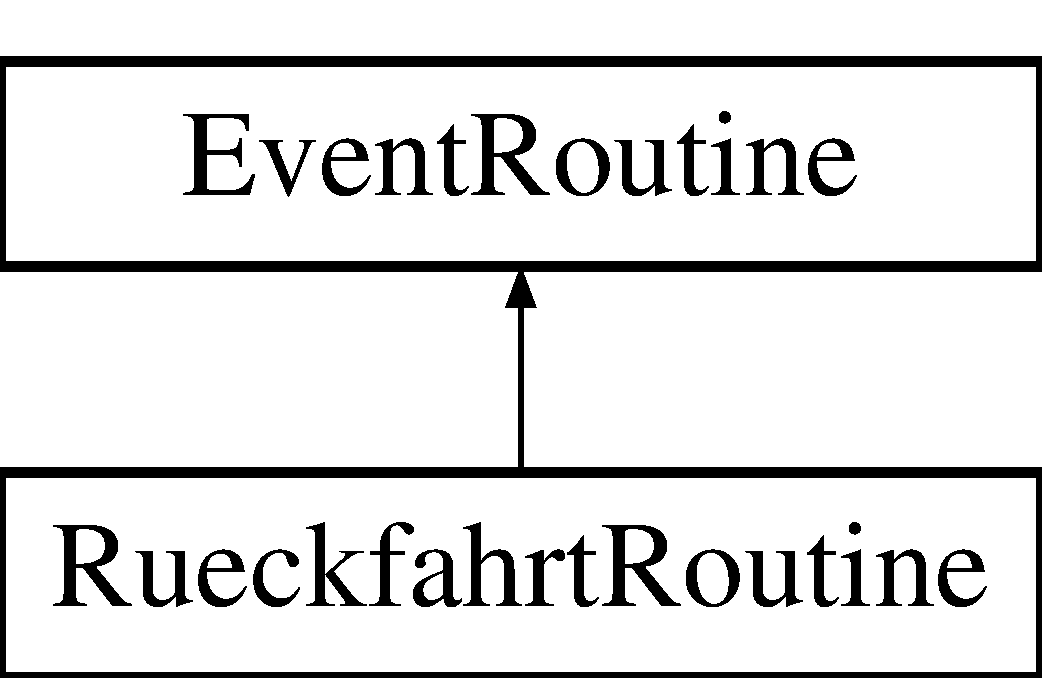
\includegraphics[height=2.000000cm]{classRueckfahrtRoutine}
\end{center}
\end{figure}
\subsection*{Öffentliche Methoden}
\begin{DoxyCompactItemize}
\item 
\hyperlink{classRueckfahrtRoutine_af906605c22d0d8fd2d002f4fa165afee}{Rueckfahrt\+Routine} (\hyperlink{classNotarzt}{Notarzt} $\ast$notarzt, \hyperlink{classEventList}{Event\+List} $\ast$event\+List, \hyperlink{classZufall}{Zufall} $\ast$random\+Generator)
\begin{DoxyCompactList}\small\item\em Konstruktor. \end{DoxyCompactList}\item 
void \hyperlink{classRueckfahrtRoutine_a7eec059994f3c958696697df05cfefe9}{execute} (\hyperlink{classEvent}{Event} $\ast$event)
\begin{DoxyCompactList}\small\item\em Spezifizierung der Zustandsänderungen. \end{DoxyCompactList}\end{DoxyCompactItemize}


\subsection{Ausführliche Beschreibung}
Routine für die Rückfahrt zur Zentrale. 

Diese Routine beschreibt die Zustandsänderungen in der Notarzt-\/\+Simulation wenn der \hyperlink{classNotarzt}{Notarzt} sich auf den Weg zurück zur Zentrale macht. 

\subsection{Beschreibung der Konstruktoren und Destruktoren}
\index{Rueckfahrt\+Routine@{Rueckfahrt\+Routine}!Rueckfahrt\+Routine@{Rueckfahrt\+Routine}}
\index{Rueckfahrt\+Routine@{Rueckfahrt\+Routine}!Rueckfahrt\+Routine@{Rueckfahrt\+Routine}}
\subsubsection[{\texorpdfstring{Rueckfahrt\+Routine(\+Notarzt $\ast$notarzt, Event\+List $\ast$event\+List, Zufall $\ast$random\+Generator)}{RueckfahrtRoutine(Notarzt *notarzt, EventList *eventList, Zufall *randomGenerator)}}]{\setlength{\rightskip}{0pt plus 5cm}Rueckfahrt\+Routine\+::\+Rueckfahrt\+Routine (
\begin{DoxyParamCaption}
\item[{{\bf Notarzt} $\ast$}]{notarzt, }
\item[{{\bf Event\+List} $\ast$}]{event\+List, }
\item[{{\bf Zufall} $\ast$}]{random\+Generator}
\end{DoxyParamCaption}
)}\hypertarget{classRueckfahrtRoutine_af906605c22d0d8fd2d002f4fa165afee}{}\label{classRueckfahrtRoutine_af906605c22d0d8fd2d002f4fa165afee}


Konstruktor. 

Abhängigkeiten werden injiziert und eine spezielle \hyperlink{classEventRoutine}{Event\+Routine} mit dem Event-\/\+Typ A\+B\+F\+A\+H\+R\+T\+\_\+\+Z\+U\+\_\+\+Z\+E\+N\+T\+R\+A\+LE wird erstellt. 

\subsection{Dokumentation der Elementfunktionen}
\index{Rueckfahrt\+Routine@{Rueckfahrt\+Routine}!execute@{execute}}
\index{execute@{execute}!Rueckfahrt\+Routine@{Rueckfahrt\+Routine}}
\subsubsection[{\texorpdfstring{execute(\+Event $\ast$event)}{execute(Event *event)}}]{\setlength{\rightskip}{0pt plus 5cm}void Rueckfahrt\+Routine\+::execute (
\begin{DoxyParamCaption}
\item[{{\bf Event} $\ast$}]{event}
\end{DoxyParamCaption}
)\hspace{0.3cm}{\ttfamily [virtual]}}\hypertarget{classRueckfahrtRoutine_a7eec059994f3c958696697df05cfefe9}{}\label{classRueckfahrtRoutine_a7eec059994f3c958696697df05cfefe9}


Spezifizierung der Zustandsänderungen. 

Die Rückfahrt des Arztes zur Zentrale ändert den Zustand des Notarztes und generiert ein neues \hyperlink{classEvent}{Event}, dass die Ankunft des Arztes in der Zentrale ankündigt. Der Zeitpunkt, wann der Arzt in der Zentrale ankommt, wird aus der stochastisch ermittelten Fahrtzeit und der aktuellen Simulationszeit berechnet. 

Implementiert \hyperlink{classEventRoutine_aede9b0fdb576a4a262ced2d7d6548c14}{Event\+Routine}.



Die Dokumentation für diese Klasse wurde erzeugt aufgrund der Dateien\+:\begin{DoxyCompactItemize}
\item 
/home/mkemp/\+Studium/\+Diskrete\+Simulation/notarzt-\/sim/source/include/Rueckfahrt\+Routine.\+h\item 
/home/mkemp/\+Studium/\+Diskrete\+Simulation/notarzt-\/sim/source/src/Rueckfahrt\+Routine.\+cpp\end{DoxyCompactItemize}

\hypertarget{classSimObject}{}\section{Sim\+Object Klassenreferenz}
\label{classSimObject}\index{Sim\+Object@{Sim\+Object}}
Klassendiagramm für Sim\+Object\+:\begin{figure}[H]
\begin{center}
\leavevmode
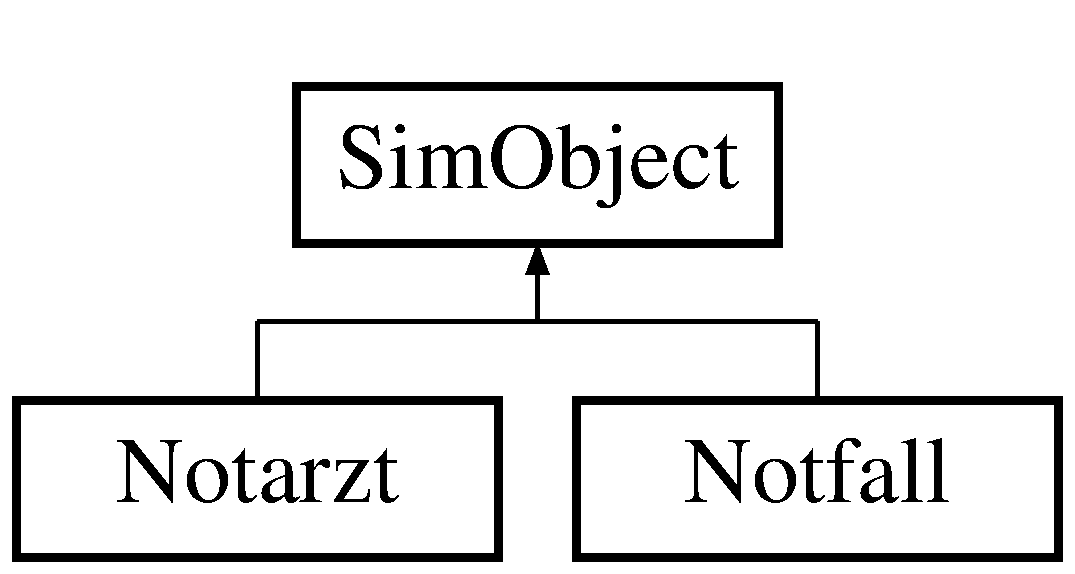
\includegraphics[height=2.000000cm]{classSimObject}
\end{center}
\end{figure}
\subsection*{Öffentliche Methoden}
\begin{DoxyCompactItemize}
\item 
virtual void {\bfseries get\+State} ()=0\hypertarget{classSimObject_a3100e6db6c86456b79351c7e6a62ec65}{}\label{classSimObject_a3100e6db6c86456b79351c7e6a62ec65}

\end{DoxyCompactItemize}


Die Dokumentation für diese Klasse wurde erzeugt aufgrund der Dateien\+:\begin{DoxyCompactItemize}
\item 
/home/mkemp/\+Studium/\+Diskrete\+Simulation/notarzt-\/sim/source/include/Sim\+Object.\+h\item 
/home/mkemp/\+Studium/\+Diskrete\+Simulation/notarzt-\/sim/source/src/Sim\+Object.\+cpp\end{DoxyCompactItemize}

\hypertarget{classSimulationManager}{}\section{Simulation\+Manager Klassenreferenz}
\label{classSimulationManager}\index{Simulation\+Manager@{Simulation\+Manager}}


Steuert die Simulation.  




{\ttfamily \#include $<$Simulation\+Manager.\+h$>$}

\subsection*{Öffentliche Methoden}
\begin{DoxyCompactItemize}
\item 
\hyperlink{classSimulationManager_a18663d0d7986354524b23a03a3ab85df}{Simulation\+Manager} (\hyperlink{classEventList}{Event\+List} $\ast$e\+List, \hyperlink{classEventRoutine}{Event\+Routine} $\ast$ro\+List\mbox{[}$\,$\mbox{]}, int num\+Routines, \hyperlink{classStateStorage}{State\+Storage} $\ast$storage)
\begin{DoxyCompactList}\small\item\em Konstruktor. \end{DoxyCompactList}\item 
void {\bfseries run} (\hyperlink{classEvent}{Event} $\ast$initla\+Events\mbox{[}$\,$\mbox{]}, int size\+Events, int end\+Time)\hypertarget{classSimulationManager_a01eb4300acb43110ca98ea8020d15cb9}{}\label{classSimulationManager_a01eb4300acb43110ca98ea8020d15cb9}

\end{DoxyCompactItemize}


\subsection{Ausführliche Beschreibung}
Steuert die Simulation. 

Objekte dieser Klasse sind verantwortlich für den grundsätlichen Ablauf einer diskreten, ereignisgesteuerten Simulation. Diese besteht aus eine Initialisierungspahse, wo die initale Ereignisliste mit den initialen Ereignissen gefüllt wird. Anschließend beginnt die Simulationsschleife zu laufen. 

\subsection{Beschreibung der Konstruktoren und Destruktoren}
\index{Simulation\+Manager@{Simulation\+Manager}!Simulation\+Manager@{Simulation\+Manager}}
\index{Simulation\+Manager@{Simulation\+Manager}!Simulation\+Manager@{Simulation\+Manager}}
\subsubsection[{\texorpdfstring{Simulation\+Manager(\+Event\+List $\ast$e\+List, Event\+Routine $\ast$ro\+List[], int num\+Routines, State\+Storage $\ast$storage)}{SimulationManager(EventList *eList, EventRoutine *roList[], int numRoutines, StateStorage *storage)}}]{\setlength{\rightskip}{0pt plus 5cm}Simulation\+Manager\+::\+Simulation\+Manager (
\begin{DoxyParamCaption}
\item[{{\bf Event\+List} $\ast$}]{e\+List, }
\item[{{\bf Event\+Routine} $\ast$}]{ro\+List\mbox{[}$\,$\mbox{]}, }
\item[{int}]{num\+Routines, }
\item[{{\bf State\+Storage} $\ast$}]{storage}
\end{DoxyParamCaption}
)}\hypertarget{classSimulationManager_a18663d0d7986354524b23a03a3ab85df}{}\label{classSimulationManager_a18663d0d7986354524b23a03a3ab85df}


Konstruktor. 



Die Dokumentation für diese Klasse wurde erzeugt aufgrund der Dateien\+:\begin{DoxyCompactItemize}
\item 
/home/mkemp/\+Studium/\+Diskrete\+Simulation/notarzt-\/sim/source/include/Simulation\+Manager.\+h\item 
/home/mkemp/\+Studium/\+Diskrete\+Simulation/notarzt-\/sim/source/src/Simulation\+Manager.\+cpp\end{DoxyCompactItemize}

\hypertarget{classStateStorage}{}\section{State\+Storage Klassenreferenz}
\label{classStateStorage}\index{State\+Storage@{State\+Storage}}
\subsection*{Öffentliche Methoden}
\begin{DoxyCompactItemize}
\item 
void {\bfseries save\+State} (int simulationszeit)\hypertarget{classStateStorage_a1de4d72e6b1fd1bdb2bca638a115412d}{}\label{classStateStorage_a1de4d72e6b1fd1bdb2bca638a115412d}

\item 
void {\bfseries register\+Notfall} (\hyperlink{classNotfall}{Notfall} $\ast$notfall)\hypertarget{classStateStorage_ab0db339611f52d600525780596f1c836}{}\label{classStateStorage_ab0db339611f52d600525780596f1c836}

\item 
void {\bfseries unregister\+Notfall} (\hyperlink{classNotfall}{Notfall} $\ast$notfall)\hypertarget{classStateStorage_a231238d0d1323f35f122758b60a5f57e}{}\label{classStateStorage_a231238d0d1323f35f122758b60a5f57e}

\item 
void {\bfseries register\+Notarzt} (\hyperlink{classNotarzt}{Notarzt} $\ast$notarzt)\hypertarget{classStateStorage_a58fbeab4cfe7baff4074e354898d5ade}{}\label{classStateStorage_a58fbeab4cfe7baff4074e354898d5ade}

\item 
void {\bfseries unregister\+Notarzt} (\hyperlink{classNotarzt}{Notarzt} $\ast$notarzt)\hypertarget{classStateStorage_aff781895425916eb0fe251ec0cccfcfe}{}\label{classStateStorage_aff781895425916eb0fe251ec0cccfcfe}

\item 
void {\bfseries check\+\_\+error} ()\hypertarget{classStateStorage_af0501a41dad1506616ed783e6181cb05}{}\label{classStateStorage_af0501a41dad1506616ed783e6181cb05}

\item 
void {\bfseries dbconnect} ()\hypertarget{classStateStorage_afaa0feafcaf5d241aefd34b53563d25e}{}\label{classStateStorage_afaa0feafcaf5d241aefd34b53563d25e}

\item 
void {\bfseries dbdisconnect} ()\hypertarget{classStateStorage_ae858cb92232b1b097364803e1677670e}{}\label{classStateStorage_ae858cb92232b1b097364803e1677670e}

\item 
void {\bfseries dbtest} ()\hypertarget{classStateStorage_a525c4f4980167fa63dc99e446a825997}{}\label{classStateStorage_a525c4f4980167fa63dc99e446a825997}

\item 
int {\bfseries max\+\_\+id\+Notarzt} ()\hypertarget{classStateStorage_a03a24b950d224309b64296757cea35c6}{}\label{classStateStorage_a03a24b950d224309b64296757cea35c6}

\item 
int {\bfseries max\+\_\+id\+Notfall} ()\hypertarget{classStateStorage_a31d513563b819d071973c2642e3bd16c}{}\label{classStateStorage_a31d513563b819d071973c2642e3bd16c}

\item 
void {\bfseries store\+Notarzt} (\hyperlink{classNotarzt}{Notarzt} $\ast$notarzt, int simulationszeit)\hypertarget{classStateStorage_aa1d8567c55db9f47d18434b33f524f73}{}\label{classStateStorage_aa1d8567c55db9f47d18434b33f524f73}

\item 
void {\bfseries store\+Notfall} (\hyperlink{classNotfall}{Notfall} $\ast$notfall, int simulationszeit)\hypertarget{classStateStorage_a3625f3b3094d88fbb516886d00f02942}{}\label{classStateStorage_a3625f3b3094d88fbb516886d00f02942}

\end{DoxyCompactItemize}


Die Dokumentation für diese Klasse wurde erzeugt aufgrund der Dateien\+:\begin{DoxyCompactItemize}
\item 
/home/mkemp/\+Studium/\+Diskrete\+Simulation/notarzt-\/sim/source/include/State\+Storage.\+h\item 
/home/mkemp/\+Studium/\+Diskrete\+Simulation/notarzt-\/sim/source/src/State\+Storage.\+cpp\end{DoxyCompactItemize}

\hypertarget{classZufall}{}\section{Zufall Klassenreferenz}
\label{classZufall}\index{Zufall@{Zufall}}
\subsection*{Öffentliche Methoden}
\begin{DoxyCompactItemize}
\item 
void {\bfseries get\+Random\+Exp\+Notruf} (int Zeitraum, vector$<$ int $>$ $\ast$vec, int $\ast$size)\hypertarget{classZufall_a0b0478a0493ac197fd447f66da4e2dec}{}\label{classZufall_a0b0478a0493ac197fd447f66da4e2dec}

\item 
int {\bfseries get\+Prio} ()\hypertarget{classZufall_a8d7735aac45ceb9a5fcce55aea5f131c}{}\label{classZufall_a8d7735aac45ceb9a5fcce55aea5f131c}

\item 
int {\bfseries versorgungszeit} (int Prio)\hypertarget{classZufall_aed840e095948ea0da9f6e80abdee4b97}{}\label{classZufall_aed840e095948ea0da9f6e80abdee4b97}

\item 
int {\bfseries get\+Stadtbezirk} ()\hypertarget{classZufall_a9388b4d00d91f5df299dc82b7ef18fb7}{}\label{classZufall_a9388b4d00d91f5df299dc82b7ef18fb7}

\item 
int {\bfseries Fahrzeit} (int Bezirk1, int Bezirk2)\hypertarget{classZufall_ae211b1e30f43f8c1f6f98f320de5a09c}{}\label{classZufall_ae211b1e30f43f8c1f6f98f320de5a09c}

\end{DoxyCompactItemize}
\subsection*{Statische öffentliche Attribute}
\begin{DoxyCompactItemize}
\item 
static int {\bfseries Bevoelkerung} \mbox{[}$\,$\mbox{]} = \{10000,30000,50000,31000,50000,10000,66000,15000,4000,1000\}\hypertarget{classZufall_a705f377c0385aae8983bc1900125bb85}{}\label{classZufall_a705f377c0385aae8983bc1900125bb85}

\item 
static int {\bfseries Bev\+Array\+Size} = 10\hypertarget{classZufall_a2282fcc0ef906d8ab1564f18fc8d02c5}{}\label{classZufall_a2282fcc0ef906d8ab1564f18fc8d02c5}

\item 
static std\+::time\+\_\+t {\bfseries now} = std\+::time(0)\hypertarget{classZufall_a453fef30bfcf43df2ac0f6a32727cec4}{}\label{classZufall_a453fef30bfcf43df2ac0f6a32727cec4}

\item 
static boost\+::random\+::mt19937 {\bfseries gen} = boost\+::random\+::mt19937(static\+\_\+cast$<$uint32\+\_\+t$>$(now))\hypertarget{classZufall_a0513d6b615dea0d472e347b8dfe566c1}{}\label{classZufall_a0513d6b615dea0d472e347b8dfe566c1}

\end{DoxyCompactItemize}


Die Dokumentation für diese Klasse wurde erzeugt aufgrund der Dateien\+:\begin{DoxyCompactItemize}
\item 
/home/mkemp/\+Studium/\+Diskrete\+Simulation/notarzt-\/sim/source/include/Zufall.\+h\item 
/home/mkemp/\+Studium/\+Diskrete\+Simulation/notarzt-\/sim/source/src/Zufall.\+cpp\end{DoxyCompactItemize}

%--- End generated contents ---

% Index
\backmatter
\newpage
\phantomsection
\clearemptydoublepage
\addcontentsline{toc}{chapter}{Index}
\printindex

\end{document}
